\documentclass[a4paper,11pt]{memoir}

\usepackage[utf8,latin1]{inputenc}
\usepackage[final]{pdfpages}
\usepackage{amsmath, amssymb}
\usepackage{graphicx}
\usepackage{color}
\usepackage{textcomp}
\usepackage{caption}
\usepackage[version=3]{mhchem}
\usepackage{url}
\usepackage{wasysym}
\usepackage{longtable}
\usepackage{afterpage}
\usepackage[hidelinks]{hyperref}
\usepackage{booktabs} 
\usepackage{colortbl} 
\usepackage{xcolor} 
\usepackage{xfrac}
\usepackage{lipsum}


%%%%%%%%%%%%%%%%%%%%%%%%%%%%%%%%%%%%%%%%
% Bibliography stuff
\usepackage[backend=bibtex8,terseinits=true,firstinits=true,natbib=true,sortcites]{biblatex}
% \usepackage[backend=bibtex8,terseinits=true,firstinits=true,natbib=true]{biblatex}

\usepackage[babel, german=quotes]{csquotes}
\AtEveryBibitem{
  \clearfield{issn}
  \clearfield{url}
  \clearfield{doi}
  \clearfield{number}
  \clearfield{day}
  \clearfield{month}
  \clearfield{endday}
  \clearfield{endmonth}
}
\DeclareFieldFormat[article]{volume}{\textbf{#1}}
\renewcommand{\cite}[1]{\textcolor{blue}{\supercite{#1}}}
\bibliography{./library.bib} 
%%%%%%%%%%%%%%%%%%%%%%%%%%%%%%%%%%%%%%


%%%%%%%%%%%%%%%%%%%%%%%%%%%%%%%%%%%%%%
% Memoir Styles
\setulmarginsandblock{3cm}{3cm}{*}
\setlrmarginsandblock{3cm}{2cm}{*}
\renewcommand{\epigraphflush}{center}
\renewcommand{\epigraphwidth}{0.9\textwidth}
\checkandfixthelayout
\chapterstyle{madsen}
\pagestyle{ruled}
\newcommand\blankpage{%
    \null
    \thispagestyle{empty}%
    \newpage}
%%%%%%%%%%%%%%%%%%%%%%%%%%%%%%%%%%%%%%


\begin{document}

\mainmatter
%
%
%
%
%
%
%
%
\thispagestyle{empty}
\pagenumbering{gobble}% Remove page numbers (and reset to 1)

\vspace*{-0.1cm}
\begin{center}
   {\Huge \textsf{Meditations on technology:\vspace{.3cm} The transcendence of the paperclip}\\}
   
    \vspace{3cm}
   {\Large \textbf{Dissertation}\\(Cumulative Dissertation)\\}
   \vspace{3cm}
   {\large for the award of the degree\\
   \textit{``PhD''}\\
    \vspace{.5cm} School of Arts and Sciences of the Miscatonic University\\
   submitted by}\\
   \vspace{3cm}
   {\Large \textbf{Angus ``Mac'' MacGyver}}\\
   \vspace{.2cm}
   {\large from Mission City, Minnesota\\
   \vspace{5cm}
   Arkham, Massachusetts 2017}
\end{center}
%
%
%
%
%
%
%
%
%
%
%
%
%
%
\newpage
\thispagestyle{empty}
\par\vspace*{\fill}

\hspace{-1cm}Thesis committee:
\begin{itemize}
 \item Dr. Spok (Thesis supervisor and 1$^\text{st}$ reviewer) \\
 \textit{Vulcan Academy of Sciences.}
 \item Dr. Charles Forbin (2$^\text{nd}$ reviewer)\\
 \textit{Head of Advanced Cybernetics, Colossus project.}
 \item Dr. Victor Frankenstein (Thesis cosupervisor)\\
 \textit{Transylvanian Institute for Experimental Medicine}
\end{itemize}

\hspace{-1cm}Further members of the examination board:
\begin{itemize}
 \item Dr. Henry Jekyll, \\
 \textit{Dept. Medicine, Miscatonic University}
 \item Dr. Julius No, \\
 \textit{Nuclear Engineering, SPECTRE}
 \item Prof. Dr. William Dyer, \\
 \textit{Dept. Geology, Miscatonic University}
\end{itemize}
\vspace{1cm}
\hspace{-.5cm}Date of oral examination: August $22^\text{nd}$, 2017
%
%
%
%
%
%
%
%
%
%
%
%
%
%
%
%
%%% NICHT MEHR NOETIG SEIT 2012!!
% \newpage
% \thispagestyle{empty}
% \vspace*{1cm}
% \hspace{-.7cm}{\Large Affidavit\vspace{1cm}\\}
% I hereby declare that this dissertation entitled ``The reconstitution of visual cortical feature selectivity \textit{in vitro}'' has been written independently and with no other sources and aids than quoted.\\
% \vspace{3cm}
% 
% \begin{flushleft}
% \begin{tabular}{ll}
% \makebox[0.1in]{\,} & \makebox[3.5in]{\hrulefill}\\
% \makebox[2.0in]{\,} & \makebox[3.5in]{Manuel Schottdorf, G\"ottingen, June 2017}\\
% \end{tabular}
% \end{flushleft}
\null
\newpage
\thispagestyle{empty}
%
%
%
%
%
%
%
%
\clearpage
\pagenumbering{arabic} %Now start numbering of pages

\vspace*{-0.15\textheight}
\tableofcontents
%
\chapter{Introduction}

\vskip-.1cm
\epigraph{``What I cannot create, I do not understand.''}{Richard Feynman\cite{Schottdorf2012}, 1988}
\vskip-.1cm
\newpage
% 
%
%
%
%
\section{Introduction}
\lipsum
Citation in the text\cite{Schottdorf2013}.
%
%
%
%
\section{Content}
%
%
\lipsum[1-1]
In the first part of this thesis is \textbf{chapter~\ref{chapter_1}}, then \textbf{chapter~\ref{chapter_2}}


%
%
\chapter{Title of Mainchapter 1}
\label{chapter_1}
%
\vskip-.1cm
\epigraph{``I have of late, (but wherefore I know not) lost all my mirth, forgone all custom of exercises; and indeed, it goes so heavily with my disposition; that this goodly frame the earth, seems to me a sterile promontory; this most excellent canopy the air, look you, this brave o'er hanging firmament, this majestical roof, fretted with golden fire: why, it appeareth no other thing to me, than a foul and pestilent congregation of vapours. What a piece of work is man, How noble in reason, how infinite in faculty, In form and moving how express and admirable, In action how like an Angel, In apprehension how like a god, The beauty of the world, The paragon of animals.''}{Hamlet\cite{Schottdorf2013}, 1601}
%
\vskip-.1cm
\section{Content}
\lipsum[1-1]
%
%
\newpage
\section{Introduction}
Every scientific text needs a good introduction.
\lipsum
%
%
%
\section{Results}
In the results, there are tables, for instance \ref{tab_1}, and figures, for instance \ref{fig1}.
%
\begin{table}
\begin{center}
\begin{tabular}{l c c c c} \hline
$\epsilon\,[\text{deg}]$  & $k_\text{pref}\,[\text{cyc}/\text{deg}]$ & $M[\text{mm}_c/\text{deg}]$ & $k_\text{pref}\,[\text{cyc}/\text{mm}_c]$ & $\lambda\,[\text{mm}_c$] \\
\hline
\rowcolor{gray!50}0 - 5     & 1.3 & 1.2 & 1.1 & 0.9 \\
5 - 10    & 0.6 & 0.5 & 1.2 & 0.8 \\
\rowcolor{gray!50} 23 [m623] & 0.7 & 0.4 & 1.8 & 0.6 \\ \hline
\end{tabular}
\caption{A good chaption}
\label{tab_1}
\end{center}
\end{table}
%
\lipsum
%
\begin{figure}
\centering
 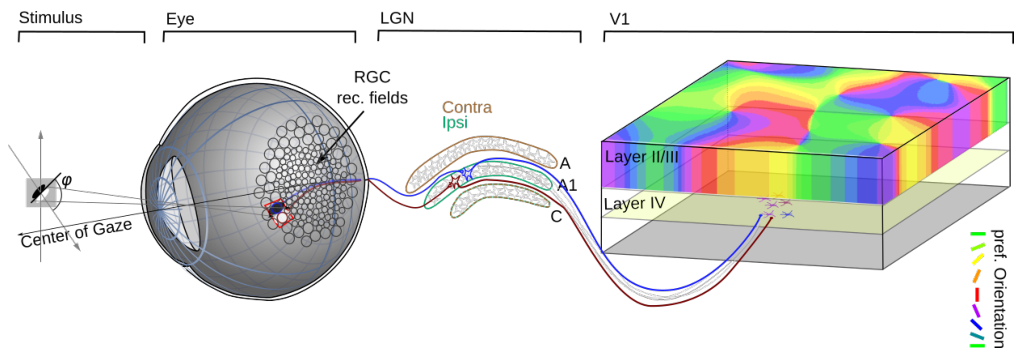
\includegraphics[width=\linewidth]{./chapter_1/fig1/fig1.pdf}
\caption{\label{fig1} \textbf{A nice figure.} \textbf{A} Try to use vector files. I recomment inkscape.}
\end{figure}





% %
% %
\chapter{Titlle of Mainchapter 2}
\label{chapter_2}
%
\vskip-.1cm
\epigraph{``Graves at my command have waked their sleepers, oped, and let 'em forth by my so potent art. But this rough magic I here abjure, and, when I have required some heavenly music, which even now I do, to work mine end upon their senses that this airy charm is for, I'll break my staff, bury it certain fathoms in the earth, and deeper than did ever plummet sound I'll drown my book.''}{Prospero\cite{Schottdorf2015}, 1601.}
%
\vskip-.1cm
\section{Content}
\lipsum[1-1]
%
%
\newpage
\section{Introduction}
\lipsum[2-3]

\section{Results}
\lipsum[4-5]



% %
%
%
\backmatter
\printbibliography
%
%
\chapter{Acknowledgements and CV}
\label{acknowledgements}
%
%
%
%
%
\section{Acknowledgements}
%
%
\lipsum[1-2]
%
%
%
%
%
%
%
\newpage
% \thispagestyle{empty}
\section{Curriculum Vit\ae}
\vspace{1cm}
%
%
{\hspace{.1cm}\textbf{Personal Details}}\vspace{.2cm}
{\color{lightgray}\hrule}
\begin{longtable}{l r}
Date of birth & \begin{minipage}[t]{0.7\textwidth}March 23, 1951 \vspace{.5cm}\end{minipage}\\[-0.3cm]
Place of birth & \begin{minipage}[t]{0.7\textwidth}Mission City, Minnesota \vspace{.5cm}\end{minipage}\\[-0.3cm]
\end{longtable}
%
\vspace{.1cm}
%
{\hspace{-.5cm}\textbf{Education}}\vspace{.2cm}
{\color{lightgray}\hrule}
\begin{longtable}{l r}
10/1986 - present & \begin{minipage}[t]{0.7\textwidth}
                    Phoenix Foundation.\vspace{.5cm}
                 \end{minipage}\\ 
10/1979 - 10/1986 & \begin{minipage}[t]{0.7\textwidth}
               Department of External Services.\vspace{.5cm}
              \end{minipage}\\
10/1975 - 10/1979 & \begin{minipage}[t]{0.7\textwidth}
                Taxi Driver, Los Angeles.\vspace{.5cm}
              \end{minipage}\\
10/1973 - 10/1975 & \begin{minipage}[t]{0.7\textwidth}
                Bomb defusing specialist, US army, Vietnam.\vspace{.5cm}
              \end{minipage}\\
10/1969 - 10/1973 & \begin{minipage}[t]{0.7\textwidth}
           B. Sc. at Western Tech in Physics and Chemistry.
           \end{minipage}\\
\end{longtable}
%
\vspace{.5cm}
%
{\hspace{-.5cm}\textbf{Additional Training}}\vspace{.2cm}
{\color{lightgray}\hrule}
\begin{longtable}{l r}
1/1974  & \begin{minipage}[t]{0.7\textwidth}Field Medic certificate.\vspace{.5cm}\end{minipage}\\
6/2011  & \begin{minipage}[t]{0.7\textwidth}Advanced diving certificate.\vspace{.5cm}\end{minipage}\\
9/1970  & \begin{minipage}[t]{0.7\textwidth}Race car driver diploma. \vspace{.5cm}\end{minipage}\\
\end{longtable}
%

%
%

\end{document}